\documentclass[11pt,psfig]{article}
\usepackage{epsfig}
\usepackage{times}
\usepackage{amssymb}
\usepackage{float}

\newcount\refno\refno=1
\def\ref{\the\refno \global\advance\refno by 1}
\def\ux{\underline{x}}
\def\uw{\underline{w}}
\def\bw{\underline{w}}
\def\ut{\underline{\theta}}
\def\umu{\underline{\mu}} 
\def\bmu{\underline{\mu}} 
\def\be{p_e^*}
\newcount\eqnumber\eqnumber=1
\def\eq{\the \eqnumber \global\advance\eqnumber by 1}
\def\eqs{\eq}
\def\eqn{\eqno(\eq)}

 \pagestyle{empty}
\def\baselinestretch{1.1}
\topmargin1in \headsep0.3in
\topmargin0in \oddsidemargin0in \textwidth6.5in \textheight8.5in
\begin{document}
\setlength{\parskip}{1.2ex plus0.3ex minus 0.3ex}


\thispagestyle{empty} \pagestyle{myheadings} \markright{G}



\title{CS 266 Homework 3}
\author{Zachary DeStefano, PhD Student, 15247592}
\date{Due Date: April 24}

\maketitle

\vfill\eject

\section*{Problem 3.11}

For this problem, it could end up not being monotone because of a concave vertex in the polygon that would cause there to be more than two intersection points in a given direction. We will thus go through each of the concave vertices and determine which directions that the polygon is not monotone in given that vertex. This will give us an interval of angles. Once we get the union of the intervals, we will see if that covers $[0,\pi]$ and if not, then the polygon is monotone for some direction. \\
\\
Here is the algorithm:\\
1. Initialize R to be empty. \\
2. For each vertex that is concave:\\
- Call the line segments through them $l$ and $l'$ \\
- Draw the lines perpendicular to $l$ and $l'$ and call them $L$ and $L'$\\
- Find the angles of $L$ and $L'$ with the x-axis and call them $\theta$ and $\theta'$. \\
- Find the min and max of $\theta$ and $\theta'$ and call them $\theta_1$ and $\theta_2$. \\
- Add $[\theta_1,\theta_2]$ to R.\\
3. Take the union of all the intervals in R. \\
4. If $[0,\pi] \subseteq R$, then the polygon is not monotone. \\
Otherwise it is monotone. 

\begin{figure}[H]
\centering
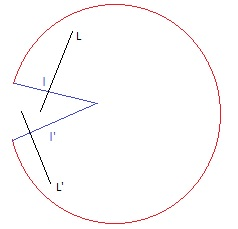
\includegraphics[height=3in]{monotone_diagram.jpg}
\caption{The non monotone directions with a concavity}
\end{figure}

Running time:\\
For each vertex, we do a constant number of operations. \\
Thus we have a total running time of $O(n)$

\newpage

\section*{Problem 3.14}

Given a simple polygon P with n vertices and a point p inside it, show
how to compute the region inside P that is visible from p.\\
\\
In the following figure, the visible region is the triangles with an X inside them. \\
\begin{figure}[H]
\centering
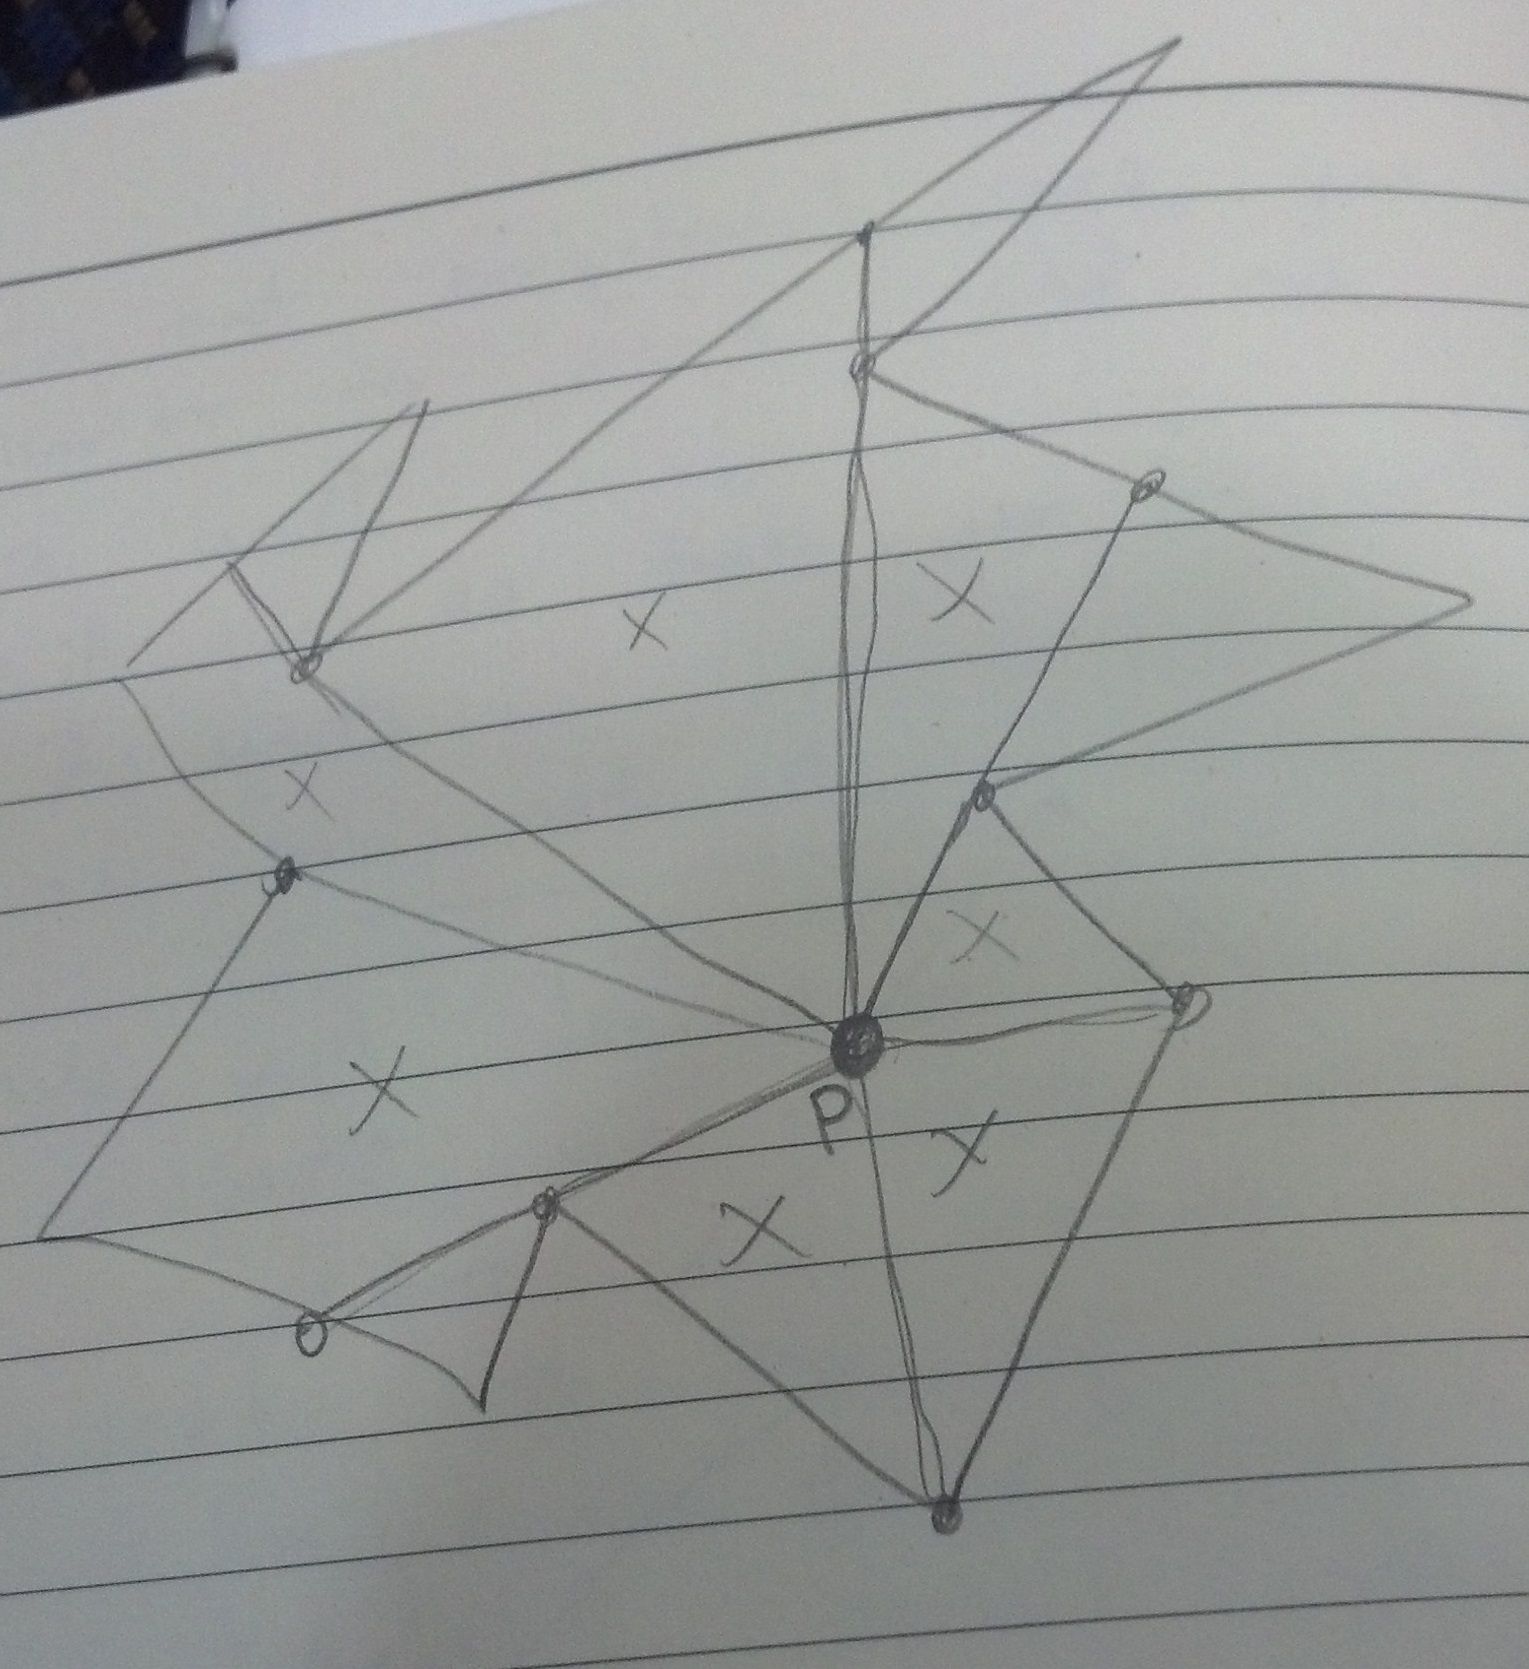
\includegraphics[height=4in]{visible_regions.jpg}
\caption{Parts of polygon visible from point p}
\end{figure}

We will want to visit the vertices in lexicographic order of the polygon. 
For visibility, we always want to make a right turn. \\
\\
Here is the algorithm:\\
1. Find the vertex $v_0$ that is closest to $P$ as it will be visible. \\
- You can take all the vertices and compute the slopes of the lines between them and $P$. \\
- You will then go through the list and find the min. \\
2. Draw a line from $v_0$ to $P$ and make $v_0$ our current point $p'$ in the traversal\\
3. For each vertex v in lexicographic order starting from $v_1$, the one after $v_0$: \\
- If vertex v takes a right turn away from $p'$, then add the line from $P$ to $v$ to our set and let $p'=v$\\
- Otherwise keep $p'$ the same and move onto the next vertex. \\
4. Go through each pair of adjacent line segments $l$ and $l'$ and if they connect vertices that are not in lexicographic order, do the following:\\
- For each line segment between the corresponding vertices for $l$ and $l'$:\\
-    - If the line extending from $l$ intersects the line segment, then extend $l$ to the line segment\\
-		 - If the line extending from $l'$ intersects the line segment, then extend $l'$ to the line segment \\
\\
Running time:\\
Step 1 takes $O(n)$ time since we are passing analyzing each vertex in a constant number of operations. \\
Step 2-3 takes $O(n)$ time since we are going in lexicographic order of the polygon. \\
Step 4 takes $O(n)$ time since we are going through each line segment in the polygon at most twice with that step. \\
The total running time is thus $O(n)$



\newpage

\section*{Problem 15.2}

If we take two points $a$ and $b$ and get their duals, $a*$ and $b*$, these lines will intersect assuming that $a$ and $b$ have different x-coordinates. \\
Denote their intersection point as $p*$\\
The dual of $p*$, which is the line $p$ in the primal plane will go through $a$ and $b$. \\
Thus, the x-coordinate of $p*$ tells us the slope of the line through $a$ and $b$. \\
\\
There is a direct relationship between slope and angle. \\
In the right half-plane the slope increases in counter-clockwise order from $-\infty$ to $\infty$. \\
In the left half-plane, the slope increases in clockwise order from $-\infty$ to $\infty$. \\
This means that if we split up the points into left and right half and then order them by the slopes, we will be able to get the radial order of the points. \\
\\
We can now translate these facts into a new algorithm:\\
1. Dualize the points\\
2. Compute the arrangement of the duals. \\
3. For each vertex v in the primal plane:\\
- Find the line v* in the dual and get its intersection points in the dual in x-coordinate order. \\
- Go through the points and put the ones corresponding to the left points into $points_{left}$ and right points into $points_{right}$. \\
- concatenate $points_{left}$ in increasing order with $points_{right}$ in decreasing order to get vertices in radial order. \\
\\
Running time:\\
Computing the arrangement takes O($n^2$). \\
Since the arrangement was computed, there is no need to sort when finding the intersection points for $v*$ thus that step is O(n). \\
This means that step 3 take O($n^2$). \\
The total running time is thus O($n^2$) which is an improvement over the last algorithm. 


\newpage

\section*{Problem 15.4}

What is the maximal number of shortest paths connecting two fixed
points among a set of n triangles in the plane?\\
\\
The visibility graph will have $V = (3n+2)$.\\
For each vertex $v$ we have $|v| \leq 3n + 2$ for the number of vertices it is connected to. \\
The max number of paths is the max number of sequences of such vertices. \\
We need to start with $s$ and end with $t$ but the vertices in the middle do not matter. \\
We end up with $(3n)!$ paths possible. \\
\\
We can tighten this when we consider that we can only be moving forward toward our point. \\
Thus any path can only go along at most 2 edges per triangle. \\
If we have to go through all n triangles and have to use two edges, then there are $2^n$ shortest paths. \\
That ends up being an upper bound. \\
\\
If the triangles are not in the way at all, then the lower bound number of paths is 1. \\
\\



\end{document}








